\documentclass[12pt,twoside,a4paper]{report}
\usepackage[a4paper,width=150mm,top=25mm,bottom=25mm,bindingoffset=6mm]{geometry}

\usepackage[utf8x]{inputenc}
\usepackage[slovak]{babel}
\usepackage{palatino,verbatim}

% Balicek pre priamu rec - \say
\usepackage{dirtytalk}

% Balicek "alltt" je to iste ako "verbatim" mod, ale navyse podporuje aj formatovacie znacky textu
\usepackage{alltt}

% Obrazky
\usepackage{graphicx}
\graphicspath{ {obr/} }

% Cislovanie obrazkov a tabuliek
\usepackage{chngcntr}
%Cisluj obrazky nezavisle od cisla kapitol/podkapitol
\counterwithout{figure}{subsection}
\counterwithout{table}{subsection}

% Referencovanie kapitol/sekcii/... podľa ich nadpisu
\usepackage{nameref}

% Tabulky s viacriadkovymi bunkami a zlucenymi bunkami
% Tabulky generujem naastrojom "http://www.tablesgenerator.com/"
\usepackage{booktabs}
\usepackage{multirow}
% LaTeX ma problemy s prikazmi cline a cmidrule, ked je babel nastaveny na slovencinu/cestinu, kvoli definicii pomlcky
% NAMIESTO POMLCKY POUZI ZNAK ZNAMIENKA MINUS "−" (plati hlavne v nazvoch nadpisov a labelov)
\usepackage{etoolbox}
\preto\tabular{\shorthandoff{-}}

%Uloz obrazok tam, kde je deklarovany
%\usepackage[subsection]{placeins}

\newcommand\sktxt[1]{\foreignlanguage{slovak}{#1}}

\begin{document}
\pagenumbering{arabic}

\setcounter{chapter}{1}
\chapter*{Internet Peering}
\paragraph{}
Andrej Šišila, Marián Vachalík

\tableofcontents

\newpage
\section{Topológia}
\paragraph{}
Budeme konfigurovať smerovacie protokoly BGP a IS-IS na topológií, ktorá je znázornená na obrázku \ref{fig:bgp_isis_topo}. Vrámci autonómnych systémov sme konfigurovali smerovacie protokoly IS-IS a BGP (iBGP). Medzi autonómnymi systémami sme konfigurovali len BGP (eBGP). IP adresácia je uvedená v tabuľke \ref{tab:ip_adresacia} a dopĺňa grafické znázornenie topológie na obrázku \ref{fig:bgp_isis_topo}. Sieť medzi smerovačmi R1 a R5 nemá mať masku \say{/48} ale \say{/30}.

\begin{figure}[!htbp]
\centering
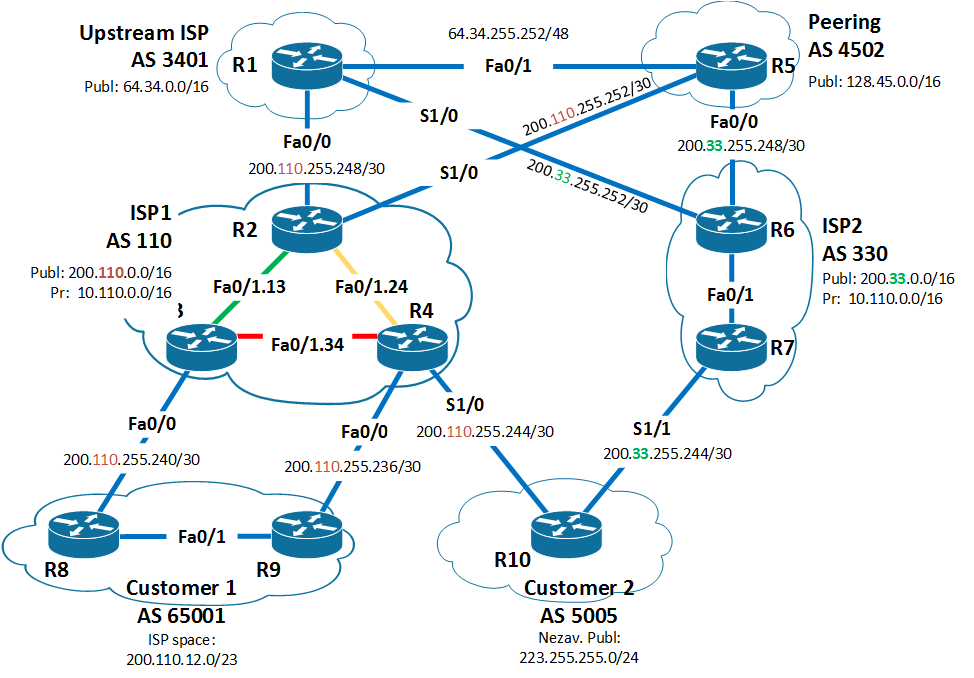
\includegraphics[width=14cm,keepaspectratio]{bgp_isis_topo}
\caption{Topológia BGP}
\label{fig:bgp_isis_topo}
\end{figure}



\begin{table}[!htbp]
\centering
\caption{IP adresácia}
\label{tab:ip_adresacia}
\begin{tabular}{|c|l|l|l|}
\hline
\textbf{Smerovač}    & \multicolumn{1}{c|}{\textbf{Rozhranie}} & \multicolumn{1}{c|}{\textbf{IP adresa}} & \multicolumn{1}{c|}{\textbf{Maska}} \\ \hline
\multirow{5}{*}{R1}  & Fa0/0                                   & 200.110.255.249                         & 255.255.255.252                     \\ \cline{2-4} 
                     & Fa0/1                                   & 64.34.255.253                           & 255.255.255.252                     \\ \cline{2-4} 
                     & S1/0                                    & 200.33.255.253                          & 255.255.255.252                     \\ \cline{2-4} 
                     & Lo0                                     & 10.255.255.1                            & 255.255.255.0                       \\ \cline{2-4} 
                     & Lo100                                   & 64.34.1.1                               & 255.255.255.128                     \\ \hline
\multirow{6}{*}{R2}  & Fa0/0                                   & 200.110.255.250                         & 255.255.255.252                     \\ \cline{2-4} 
                     & Fa0/1.23                                & 10.110.23.2                             & 255.255.255.0                       \\ \cline{2-4} 
                     & Fa0/1.24                                & 10.110.24.2                             & 255.255.255.0                       \\ \cline{2-4} 
                     & S1/0                                    & 200.110.255.253                         & 255.255.255.252                     \\ \cline{2-4} 
                     & Lo0                                     & 10.255.255.2                            & 255.255.255.0                       \\ \cline{2-4} 
                     & Lo100                                   & 200.110.0.2                             & 255.255.255.128                     \\ \hline
\multirow{5}{*}{R3}  & Fa0/0                                   & 200.110.255.241                         & 255.255.255.252                     \\ \cline{2-4} 
                     & Fa0/1.23                                & 10.110.23.3                             & 255.255.255.0                       \\ \cline{2-4} 
                     & Fa0/1.34                                & 10.110.34.3                             & 255.255.255.0                       \\ \cline{2-4} 
                     & Lo0                                     & 10.255.255.3                            & 255.255.255.0                       \\ \cline{2-4} 
                     & Lo100                                   & 200.110.0.133                           & 255.255.255.128                     \\ \hline
\multirow{6}{*}{R4}  & Fa0/0                                   & 200.110.255.237                         & 255.255.255.252                     \\ \cline{2-4} 
                     & Fa0/1.24                                & 10.110.24.4                             & 255.255.255.0                       \\ \cline{2-4} 
                     & Fa0/1.34                                & 10.110.34.4                             & 255.255.255.0                       \\ \cline{2-4} 
                     & S1/0                                    & 200.110.255.245                         & 255.255.255.252                     \\ \cline{2-4} 
                     & Lo0                                     & 10.255.255.4                            & 255.255.255.0                       \\ \cline{2-4} 
                     & Lo100                                   & 200.110.1.4                             & 255.255.255.128                     \\ \hline
\multirow{5}{*}{R5}  & Fa0/0                                   & 200.33.255.249                          & 255.255.255.252                     \\ \cline{2-4} 
                     & Fa0/1                                   & 10.100.15.2                             & 255.255.255.252                     \\ \cline{2-4} 
                     & S1/0                                    & 200.110.255.254                         & 255.255.255.252                     \\ \cline{2-4} 
                     & Lo0                                     & 10.255.255.5                            & 255.255.255.0                       \\ \cline{2-4} 
                     & Lo100                                   & 128.45.5.5                              & 255.255.255.128                     \\ \hline
\multirow{5}{*}{R6}  & Fa0/0                                   & 200.33.255.250                          & 255.255.255.252                     \\ \cline{2-4} 
                     & Fa0/1                                   & 10.110.67.6                             & 255.255.255.0                       \\ \cline{2-4} 
                     & S1/0                                    & 200.33.255.254                          & 255.255.255.252                     \\ \cline{2-4} 
                     & Lo0                                     & 10.255.255.6                            & 255.255.255.0                       \\ \cline{2-4} 
                     & Lo100                                   & 200.33.6.6                              & 255.255.255.128                     \\ \hline
\multirow{4}{*}{R7}  & Fa0/1                                   & 10.110.67.7                             & 255.255.255.0                       \\ \cline{2-4} 
                     & S1/1                                    & 200.33.255.245                          & 255.255.255.252                     \\ \cline{2-4} 
                     & Lo0                                     & 10.255.255.7                            & 255.255.255.0                       \\ \cline{2-4} 
                     & Lo100                                   & 200.33.7.7                              & 255.255.255.128                     \\ \hline
\multirow{4}{*}{R8}  & Fa0/0                                   & 200.110.255.242                         & 255.255.255.252                     \\ \cline{2-4} 
                     & Fa0/1                                   & 10.110.89.8                             & 255.255.255.0                       \\ \cline{2-4} 
                     & Lo0                                     & 10.255.255.8                            & 255.255.255.0                       \\ \cline{2-4} 
                     & Lo100                                   & 200.110.12.8                            & 255.255.255.128                     \\ \hline
\multirow{4}{*}{R9}  & Fa0/0                                   & 200.110.255.238                         & 255.255.255.252                     \\ \cline{2-4} 
                     & Fa0/1                                   & 10.110.89.9                             & 255.255.255.0                       \\ \cline{2-4} 
                     & Lo0                                     & 10.255.255.9                            & 255.255.255.0                       \\ \cline{2-4} 
                     & Lo100                                   & 200.110.13.9                            & 255.255.255.128                     \\ \hline
\multirow{4}{*}{R10} & S1/0                                    & 200.110.255.246                         & 255.255.255.252                     \\ \cline{2-4} 
                     & S1/1                                    & 200.33.255.246                          & 255.255.255.252                     \\ \cline{2-4} 
                     & Lo0                                     & 10.255.255.10                           & 255.255.255.0                       \\ \cline{2-4} 
                     & Lo100                                   & 223.255.255.10                          & 255.255.255.128                     \\ \hline
\end{tabular}
\end{table}


% Novu kapitolu davam na novu stranu, lebo bez toho mi zobrazuje tabulku v dalsej kapitole, kde ale tabulka nepatri.
\newpage

\section{Úlohy}
\subsection{Použiť IGP IS−IS (L2 only) single area dizajn, priame p2p prepojenia}
\subsection{Zabezpečiť plnú konektivitu prostredníctvom iBGP alebo eBGP protokolov pre zákaznícké a internetové smerovacie záznamy}
\subsection{Distribúcia internetových statických smerovacích záznamov z AS3401, AS4502 a zákaznických smerovacích záznamov z AS65001, AS5005, AS330}
\subsection{Sumarizácia}


\subsubsection{Popis}
\paragraph{}
V celej topológií používame smerovací protokol BGP. Vnútri všetkých autonómnych systémov navyše používame smerovací protokol IS-IS. Subrozhranie “.13” (VLAN 13) sme premenovali na “.23” (VLAN 23), lebo sieť je medzi smerovačmi R2 a R3 (23), a nie medzi R1 a R3 (13).

\paragraph{}
Najprv sme linky medzi autonómnymi systémami šírili cez IS-IS. Neskôr sa toto ukázalo ako nevhodné riešenie, pretože \say{flappovacie} linky u zákazníkov môžu spôsobiť nestabilitu siete. Preto boli rozhrania medzi AS odstranené z IS-IS príkazmi uvedenými nižšie.

\noindent
{\fontfamily{qcr}\selectfont
\begin{small}
\begin{alltt}
int <nazov_interfaceu>
  no ip router isis
router isis
  no passive-interface <nazov_interfaceu>
  no redistribute-connected
\end{alltt}
\end{small}
}

\paragraph{}
Na smerovačoch sme vytvorili dve virtuálne rozhrania: Loopback0 a Loopback100. Loopback0 mal IP adresu v tvare \say{10.255.255.X} s maskou \say{/32}, kde X je číslo smerovača. Router-ID sme nastavili na IP adresu rozhrania Loopback0. V rámci BGP sme ho nastavovali príkazom \say{bgp router-id 10.255.255.X}. Pokiaľ sa Router ID v BGP nenastaví hneď na začiatku, jeho zmena spôsobí rozpad BGP spojenia, ktoré sa po chvíli (rádovo v desiatkach sekúnd) obnoví.

\paragraph{}
Loopback100 mal IP adresu z verejného rozsahu príslušnej autonómnej oblasti s maskou \say{/25}. Verejné adresné rozsahy na Loopback100 rozhraniach sme sumarizovali pre každú AS príkazom \say{aggregate-address}. S AS 65001 vznikol problém so sumarizáciou ich verejného rozsahu na smerovačoch R3 a R4, lebo, lebo \say{Customer 1} (AS 65001) mal používal podrozsah verejných adries \say{ISP1} (AS 110). Ak by sme na R3 a R4 vykonali sumarizáciu verejných rozsahov pre Loopback100 v AS 110, spôsobilo by to, že \say{next-hop} adresa pre Loopback100 v AS 65001 by bol \say{Null0} t.j. paket by bol zahodený. Na R4 sme sumarizáciu nerobili, pretože keby vypadla linka medzi R2 a R3, do AS 65001 by sme išli cez R4, a pokiaľ by mal R4 spomenutú sumárnu cestu, vznikol by ten istý problém s konektivitou.

\paragraph{}
V rámci BGP sme každému smerovaču nakonfigurovali siete, s ktorými susedí resp. na ktoré je priamo pripojený príkazom \say{neighbor}. Podľa toho, či sa susediaca sieť nachádza v AS s rovnakým číslom ako je ASN daného smerovača, použije sa iBGP, inak sa použije eBGP. 

\paragraph{}
Siete obidvoch Loopback rozhraní sme ohlasovali príkazom \say{network} v rámci BGP. Potom sme pre ne použili príkaz \say{update-source}, ktorý slúži na prepísanie zdrojovej IP adresy na Loopback0. Keďže sme Loopback0 ohlásili príkazom \say{network}, susediace smerovače mu budú môcť odpovedať. Zdrojová adresa sa potom použije na otvorenie BGP spojenia medzi susednými smerovačmi. Loopback0 používame aj kvôli tomu, že bude vždy zapnutý, takže BGP spojenie bude stále aktívne.

\paragraph{}
Pokiaľ boli v AS viac ako dva smerovače, museli sme pridať príkaz \say{next-hop-self}, aby sme zaistili konektivitu medzi AS. Príkaz \say{next-hop-self} sa používa, keď sa BGP smerovač v jednom AS dozvie o ceste z iného AS cez eBGP a dá o tejto ceste vedieť zvyšným iBGP smerovačom v rámci svojho AS. Aby mohol iBGP smerovač získať konektivitu do tejto siete, použijeme na eBGP príkaz \say{next-hop-self}, ktorý namiesto toho, aby preposielal prefix s \say{next-hop} adresou zo siete medzi operátormi, prepíše \say{next-hop} adresu na svoj Loopback0. iBGP smerovač tak získa konektivitu do danej siete cez hraničný eBGP smerovač vo svojej oblasti. Keby sme tak neurobili, iBGP smerovač by sa nemohol dostať do siete v susednom AS, keď k nej nemá eBGP spojenie a z dôvodu bezpečnosti sme linky medzi AS neohlasovali príkazom \say{network}.


\subsubsection{Konfigurácia}

\noindent
{\fontfamily{qcr}\selectfont
\begin{small}
\begin{alltt}
R1
ena
conf t
hostname R1
no ip domain-lookup
username admin privil 15 secret admin
line con 0
  login local
  logging syn
  exec-time 120
line vty 0 15
  privilege level 15
  no login
int f0/0
  ip addr 200.110.255.249 255.255.255.252
  no shut
int f0/1
  ip addr 64.34.255.253 255.255.255.252
  no shut
int s1/0
  ip addr 200.33.255.253 255.255.255.252
  no shut
int lo0
  ip addr 10.255.255.1 255.255.255.255
  no shut
int lo100
  ip addr 64.34.1.1 255.255.255.128
  no shut
router bgp 3401
  bgp router-id 10.255.255.1
  neighbor 64.34.255.254 remote-as 4502
  neighbor 200.33.255.254 remote-as 330
  neighbor 200.110.255.250 remote-as 110
  network 10.255.255.1 mask 255.255.255.255
  network 64.34.1.0 mask 255.255.255.128
  aggregate-address 64.34.0.0 255.255.0.0 summary-only
  no auto-summary
  no sync
  bgp log-neighbor-changes



R2
ena
conf t
hostname R2
no ip domain-lookup
username admin privil 15 secret admin
line con 0
  login local
  logging syn
  exec-time 120
line vty 0 15
  privilege level 15
  no login
int f0/0
  ip addr 200.110.255.250 255.255.255.252
  no shut
int f0/1
  no ip add
  isis network point-to-point
  no sh
int f0/1.23
  encap dot1q 23
  ip addr 10.110.23.2 255.255.255.0
  ip router isis
int f0/1.24
  encap dot1q 24
  ip addr 10.110.24.2 255.255.255.0
  ip router isis
int s1/0
  ip addr 200.110.255.253 255.255.255.252
  no shut
int lo0
  ip addr 10.255.255.2 255.255.255.255
  ip router isis
  no shut
int lo100
  ip addr 200.110.0.2 255.255.255.128
  ip router isis
  no shut
router isis
  net 49.0001.0102.5525.5002.00
  passive-interface lo0
  passive-interface lo100
  redistribute static
  is-type level-2
  metric-style wide
  exit
router bgp 110
  bgp router-id 10.255.255.2
  neighbor 10.255.255.3 remote-as 110
  neighbor 10.255.255.3 update-source lo0
  neighbor 10.255.255.3 next-hop-self
  neighbor 10.255.255.4 remote-as 110
  neighbor 10.255.255.4 update-source lo0
  neighbor 10.255.255.4 next-hop-self
  neighbor 200.110.255.249 remote-as 3401
  neighbor 200.110.255.254 remote-as 4502
  network 10.255.255.2 mask 255.255.255.255
  network 200.110.0.0 mask 255.255.255.128
  aggregate-address 200.110.0.0 255.255.0.0 summary-only
  no auto-summary
  no sync
  bgp log-neighbor-changes



R3
ena
conf t
hostname R3
no ip domain-lookup
username admin privil 15 secret admin
line con 0
  login local
  logging syn
  exec-time 120
line vty 0 15
  privilege level 15
  no login
int f0/0
  ip addr 200.110.255.241 255.255.255.252
  no shut
int f0/1
  no ip addr
  isis network point-to-point
  no shut
int f0/1.23
  encap dot1q 23
  ip addr 10.110.23.3 255.255.255.0
  ip router isis
int f0/1.34
  encap dot1q 34
  ip addr 10.110.34.3 255.255.255.0
  ip router isis
int lo0
  ip addr 10.255.255.3 255.255.255.255
  ip router isis
  no shut
int lo100
  ip addr 200.110.0.133 255.255.255.128
  ip router isis
  no shut
router isis
  net 49.0001.0102.5525.5003.00
  passive-interface lo0
  passive-interface lo100
  redistribute static
  is-type level-2
  metric-style wide
  exit
router bgp 110
  bgp router-id 10.255.255.3
  neighbor 10.255.255.2 remote-as 110
  neighbor 10.255.255.2 update-source lo0
  neighbor 10.255.255.2 next-hop-self
  neighbor 10.255.255.4 remote-as 110
  neighbor 10.255.255.4 update-source lo0
  neighbor 10.255.255.4 next-hop-self
  neighbor 200.110.255.242 remote-as 65001
  network 10.255.255.3 mask 255.255.255.255
  network 200.110.0.128 mask 255.255.255.128
  no auto-summary
  no sync
  bgp log-neighbor-changes




R4
ena
conf t
hostname R4
no ip domain-lookup
username admin privil 15 secret admin
line con 0
  login local
  logging syn
  exec-time 120
line vty 0 15
  privilege level 15
  no login
int f0/0
  ip addr 200.110.255.237 255.255.255.252
  no shut
int f0/1
  no ip addr
  isis network point-to-point
  no sh
int f0/1.24
  encap dot1q 24
  ip addr 10.110.24.4 255.255.255.0
  ip router isis
int f0/1.34
  encap dot1q 34
  ip addr 10.110.34.4 255.255.255.0
  ip router isis
int s1/0
  ip addr 200.110.255.245 255.255.255.252
  no shut
int lo0
  ip addr 10.255.255.4 255.255.255.255
  ip router isis
  no shut
int lo100
  ip addr 200.110.1.4 255.255.255.128
  ip router isis
  no shut
router isis
  net 49.0001.0102.5525.5004.00
  passive-interface lo0
  passive-interface lo100
  redistribute static
  is-type level-2
  metric-style wide
  exit
router bgp 110
  bgp router-id 10.255.255.4
  neighbor 10.255.255.2 remote-as 110
  neighbor 10.255.255.2 update-source lo0
  neighbor 10.255.255.2 next-hop-self
  neighbor 10.255.255.3 remote-as 110
  neighbor 10.255.255.3 update-source lo0
  neighbor 10.255.255.3 next-hop-self
  neighbor 200.110.255.238 remote-as 65001
  neighbor 200.110.255.246 remote-as 5005
  network 10.255.255.4 mask 255.255.255.255
  network 200.110.1.0 mask 255.255.255.128
  no auto-summary
  no sync
  bgp log-neighbor-changes


R5
ena
conf t
hostname R5
no ip domain-lookup
username admin privil 15 secret admin
line con 0
  login local
  logging syn
  exec-time 120
line vty 0 15
  privilege level 15
  no login
int f0/0
  ip addr 200.33.255.249 255.255.255.252
  no shut
int f0/1
  ip addr 64.34.255.254 255.255.255.252
  no shut
int s1/0
  ip addr 200.110.255.254 255.255.255.252
  no shut
int lo0
  ip addr 10.255.255.5 255.255.255.255
  no shut
int lo100
  ip addr 128.45.5.5 255.255.255.128
  no shut
router bgp 4502
  bgp router-id 10.255.255.5
  neighbor 200.33.255.250 remote-as 330
  neighbor 200.110.255.253 remote-as 110
  neighbor 64.34.255.253 remote-as 3401
  network 10.255.255.5 mask 255.255.255.255
  network 128.45.5.0 mask 255.255.255.128
  aggregate-address 128.45.0.0 255.255.0.0 summary-only
  no auto-summary
  no sync
  bgp log-neighbor-changes




R6
ena
conf t
hostname R6
no ip domain-lookup
username admin privil 15 secret admin
line con 0
  login local
  logging syn
  exec-time 120
line vty 0 15
  privilege level 15
  no login
int f0/0
  ip addr 200.33.255.250 255.255.255.252
  no shut
int f0/1
  ip addr 10.110.67.6 255.255.255.0
  ip router isis
  isis network point-to-point
  no shut
int s1/0
  ip addr 200.33.255.254 255.255.255.252
  no shut
int lo0
  ip addr 10.255.255.6 255.255.255.255
  ip router isis
  no shut
int lo100
  ip add 200.33.6.6 255.255.255.128
  ip router isis
router isis
  net 49.0001.0102.5525.5006.00
  passive-interface lo0
  passive-interface lo100
  redistribute static
  is-type level-2
  metric-style wide
  exit
router bgp 330
  bgp router-id 10.255.255.6
  neighbor 10.255.255.7 remote-as 330
  neighbor 10.255.255.7 update-source lo0
  neighbor 10.255.255.7 next-hop-self
  neighbor 200.33.255.253 remote-as 3401
  neighbor 200.33.255.249 remote-as 4502
  network 10.255.255.6 mask 255.255.255.255
  network 200.33.6.0 mask 255.255.255.128
  aggregate-address 200.33.0.0 255.255.0.0 summary-only
  no auto-summary
  no sync
  bgp log-neighbor-changes



R7
ena
conf t
hostname R7
no ip domain-lookup
username admin privil 15 secret admin
line con 0
  login local
  logging syn
  exec-time 120
line vty 0 15
  privilege level 15
  no login
int f0/1
  ip addr 10.110.67.7 255.255.255.0
  ip router isis
  isis network point-to-point
  no shut
int s1/1
  ip addr 200.33.255.245 255.255.255.252
  no shut
int lo0
  ip addr 10.255.255.7 255.255.255.255
  ip router isis
  no shut
int lo100
  ip addr 200.33.7.7 255.255.255.128
  ip router isis
  no shut
router isis
  net 49.0001.0102.5525.5007.00
  passive-interface lo0
  passive-interface lo100
  redistribute static
  is-type level-2
  metric-style wide
  exit
router bgp 330
  bgp router-id 10.255.255.7
  neighbor 10.255.255.6 remote-as 330
  neighbor 10.255.255.6 update-source lo0
  neighbor 10.255.255.6 next-hop-self
  neighbor 200.33.255.246 remote-as 5005
  network 10.255.255.7 mask 255.255.255.255
  network 200.33.7.0 255.255.255.128
  aggregate-address 200.33.0.0 255.255.0.0 summary-only
  no auto-summary
  no sync
  bgp log-neighbor-changes




R8
ena
conf t
hostname R8
no ip domain-lookup
username admin privil 15 secret admin
line con 0
  login local
  logging syn
  exec-time 120
line vty 0 15
  privilege level 15
  no login
int f0/0
  ip addr 200.110.255.242 255.255.255.252
  no shut
int f0/1
  ip addr 10.110.89.8 255.255.255.0
  ip router isis
  isis network point-to-point
  no shut
int lo0
  ip addr 10.255.255.8 255.255.255.255
  ip router isis
  no shut
int lo100
  ip add 200.110.12.8 255.255.255.128
  ip router isis
router isis
  net 49.0001.0102.5525.5008.00
  passive-interface lo0
  passive-interface lo100
  redistribute static
  is-type level-2
  metric-style wide
  exit
router bgp 65001
  bgp router-id 10.255.255.8
  neighbor 10.255.255.9 remote-as 65001
  neighbor 10.255.255.9 update-source lo0
  neighbor 200.110.255.241 remote-as 110
  network 10.255.255.8 mask 255.255.255.255
  network 200.110.12.0 mask 255.255.255.128
  aggregate-address 200.110.12.0 255.255.254.0 summary-only
  no auto-summary
  no sync
  bgp log-neighbor-changes





R9
ena
conf t
hostname R9
no ip domain-lookup
username admin privil 15 secret admin
line con 0
  login local
  logging syn
  exec-time 120
line vty 0 15
  privilege level 15
  no login
int f0/0
  ip addr 200.110.255.238 255.255.255.252
  no sh
int f0/1
  ip addr 10.110.89.9 255.255.255.0
  ip router isis
  isis network point-to-point
  no shut
int lo0
  ip addr 10.255.255.9 255.255.255.255
  ip router isis
  no shut
int lo100
  ip addr 200.110.13.9 255.255.255.128
  ip router isis
  no shut
router isis
  net 49.0001.0102.5525.5009.00
  passive-interface lo0
  passive-interface lo100
  redistribute static
  is-type level-2
  metric-style wide
  exit
router bgp 65001
  bgp router-id 10.255.255.9
  neighbor 10.255.255.8 remote-as 65001
  neighbor 10.255.255.8 update-source lo0
  neighbor 200.110.255.237 remote-as 110
  network 10.255.255.9 mask 255.255.255.255
  network 200.110.13.0 mask 255.255.255.128
  aggregate-address 200.110.12.0 255.255.254.0 summary-only
  no auto-summary
  no sync
  bgp log-neighbor-changes




R10
ena
conf t
hostname R10
no ip domain-lookup
username admin privil 15 secret admin
line con 0
  login local
  logging syn
  exec-time 120
line vty 0 15
  privilege level 15
  no login
int s1/0
  ip addr 200.110.255.246 255.255.255.252
  no shut
int s1/1
  ip addr 200.33.255.246 255.255.255.252
  no shut
int lo0
  ip addr 10.255.255.10 255.255.255.255
  no shut
int lo100
  ip addr 223.255.255.10 255.255.255.128
  no shut
router bgp 5005
  bgp router-id 10.255.255.10
  neighbor 200.110.255.245 remote-as 110
  neighbor 200.33.255.245 remote-as 330
  network 10.255.255.10 mask 255.255.255.255
  network 223.255.255.0 mask 255.255.255.128
  aggregate-address 223.255.255.0 255.255.255.0 summary-only
  no auto-summary
  no sync
  bgp log-neighbor-changes

\end{alltt}
\end{small}
}


\subsubsection{Overenie}
\paragraph{}
Kontrola, že vnútorný smerovací protokol IS-IS neohlasuje žiadne siete medzi operátormi, a že s

\paragraph{}
Nižšie uvádzame výpisy príkazov \say{show ip bgp} a \say{show ip route} pred odstránením liniek.

\noindent
{\fontfamily{qcr}\selectfont
\begin{small}
\begin{alltt}
R1#sh ip bgp              
BGP table version is 23, local router ID is 64.34.1.1
Status codes: s suppressed, d damped, h history, * valid, > best, i - internal,
              r RIB-failure, S Stale
Origin codes: i - IGP, e - EGP, ? - incomplete

   Network          Next Hop            Metric LocPrf Weight Path
*> 10.255.255.1/32  0.0.0.0                  0         32768 i
*  10.255.255.2/32  64.34.255.254                          0 4502 110 i
*>                  200.110.255.250          0             0 110 i
*  10.255.255.3/32  64.34.255.254                          0 4502 110 i
*>                  200.110.255.250                        0 110 i
*  10.255.255.4/32  64.34.255.254                          0 4502 110 i
*>                  200.110.255.250                        0 110 i
*  10.255.255.5/32  200.110.255.250                        0 110 4502 i
*                   200.33.255.254                         0 330 4502 i
*>                  64.34.255.254            0             0 4502 i
*  10.255.255.6/32  200.110.255.250                        0 110 4502 330 i
*                   64.34.255.254                          0 4502 330 i
*>                  200.33.255.254           0             0 330 i
*  10.255.255.7/32  200.110.255.250                        0 110 4502 330 i
*                   64.34.255.254                          0 4502 330 i
*>                  200.33.255.254                         0 330 i
*  10.255.255.8/32  64.34.255.254                          0 4502 110 65001 i
   Network          Next Hop            Metric LocPrf Weight Path
*                   200.33.255.254                         0 330 4502 110 65001 i
*>                  200.110.255.250                        0 110 65001 i
*  10.255.255.9/32  64.34.255.254                          0 4502 110 65001 i
*                   200.33.255.254                         0 330 4502 110 65001 i
*>                  200.110.255.250                        0 110 65001 i
*  10.255.255.10/32 64.34.255.254                          0 4502 110 5005 i
*                   200.110.255.250                        0 110 5005 i
*>                  200.33.255.254                         0 330 5005 i
*> 64.34.1.0/25     0.0.0.0                  0         32768 i
*  128.45.5.0/25    200.110.255.250                        0 110 4502 i
*                   200.33.255.254                         0 330 4502 i
*>                  64.34.255.254            0             0 4502 i
*  200.33.6.0/25    64.34.255.254                          0 4502 330 i
*>                  200.33.255.254           0             0 330 i
*  200.33.7.0/25    64.34.255.254                          0 4502 330 i
*>                  200.33.255.254                         0 330 i
*  200.110.0.0/25   200.33.255.254                         0 330 4502 110 i
*                   64.34.255.254                          0 4502 110 i
*>                  200.110.255.250          0             0 110 i
*  200.110.0.128/25   200.33.255.254                         0 330 4502 110 i
   Network          Next Hop            Metric LocPrf Weight Path
*                   64.34.255.254                          0 4502 110 i
*>                  200.110.255.250                        0 110 i
*> 200.110.1.0/25   200.110.255.250                        0 110 i
*                   64.34.255.254                          0 4502 110 i
*                   200.33.255.254                         0 330 4502 110 i
*  200.110.12.0/25  200.33.255.254                         0 330 4502 110 65001 i
*                   64.34.255.254                          0 4502 110 65001 i
*>                  200.110.255.250                        0 110 65001 i
*  200.110.13.0/25  200.33.255.254                         0 330 4502 110 65001 i
*                   64.34.255.254                          0 4502 110 65001 i
*>                  200.110.255.250                        0 110 65001 i
*  223.255.255.0/25 64.34.255.254                          0 4502 330 5005 i
*                   200.110.255.250                        0 110 5005 i
*>                  200.33.255.254                         0 330 5005 i


-------------------------------------------------------------------------------------


R1#sh ip route            
Codes: C - connected, S - static, R - RIP, M - mobile, B - BGP
       D - EIGRP, EX - EIGRP external, O - OSPF, IA - OSPF inter area 
       N1 - OSPF NSSA external type 1, N2 - OSPF NSSA external type 2
       E1 - OSPF external type 1, E2 - OSPF external type 2
       i - IS-IS, su - IS-IS summary, L1 - IS-IS level-1, L2 - IS-IS level-2
       ia - IS-IS inter area, * - candidate default, U - per-user static route
       o - ODR, P - periodic downloaded static route

Gateway of last resort is not set

     200.110.1.0/25 is subnetted, 1 subnets
B       200.110.1.0 [20/0] via 200.110.255.250, 00:06:48
     200.33.6.0/25 is subnetted, 1 subnets
B       200.33.6.0 [20/0] via 200.33.255.254, 00:08:41
     223.255.255.0/25 is subnetted, 1 subnets
B       223.255.255.0 [20/0] via 200.33.255.254, 00:11:55
     200.33.7.0/25 is subnetted, 1 subnets
B       200.33.7.0 [20/0] via 200.33.255.254, 00:09:14
     64.0.0.0/8 is variably subnetted, 2 subnets, 2 masks
C       64.34.255.252/30 is directly connected, FastEthernet0/1
C       64.34.1.0/25 is directly connected, Loopback1
     200.110.255.0/30 is subnetted, 1 subnets
C       200.110.255.248 is directly connected, FastEthernet0/0
     200.33.255.0/30 is subnetted, 1 subnets
C       200.33.255.252 is directly connected, Serial1/0
     200.110.0.0/25 is subnetted, 1 subnets
B       200.110.0.0 [20/0] via 200.110.255.250, 00:10:45
     200.110.0.128/25 is subnetted, 1 subnets
B       200.110.0.128 [20/0] via 200.110.255.250, 00:07:52
     200.110.12.0/25 is subnetted, 1 subnets
B       200.110.12.0 [20/0] via 200.110.255.250, 00:10:14
     128.45.0.0/25 is subnetted, 1 subnets
B       128.45.5.0 [20/0] via 64.34.255.254, 00:07:22
     200.110.13.0/25 is subnetted, 1 subnets
B       200.110.13.0 [20/0] via 200.110.255.250, 00:11:15
     10.0.0.0/32 is subnetted, 10 subnets
B       10.255.255.10 [20/0] via 200.33.255.254, 00:18:19
B       10.255.255.8 [20/0] via 200.110.255.250, 00:18:19
B       10.255.255.9 [20/0] via 200.110.255.250, 00:18:19
B       10.255.255.2 [20/0] via 200.110.255.250, 00:21:55
B       10.255.255.3 [20/0] via 200.110.255.250, 00:20:22
C       10.255.255.1 is directly connected, Loopback0
B       10.255.255.6 [20/0] via 200.33.255.254, 00:19:22
B       10.255.255.7 [20/0] via 200.33.255.254, 00:18:52
B       10.255.255.4 [20/0] via 200.110.255.250, 00:19:53
B       10.255.255.5 [20/0] via 64.34.255.254, 00:19:36
\end{alltt}
\end{small}
}

\paragraph{}
Nižšie uvádzame výpisy príkazov \say{show ip bgp} a \say{show ip route} po odstránení liniek prikazmi uvedenými v časti \say{Popis}.

\noindent
{\fontfamily{qcr}\selectfont
\begin{small}
\begin{alltt}
R1#show ip bgp
BGP table version is 63, local router ID is 64.34.1.1
Status codes: s suppressed, d damped, h history, * valid, > best, i - internal,
              r RIB-failure, S Stale
Origin codes: i - IGP, e - EGP, ? - incomplete

   Network          Next Hop            Metric LocPrf Weight Path
*> 10.255.255.1/32  0.0.0.0                  0         32768 i
*  10.255.255.2/32  64.34.255.254                          0 4502 110 i
*>                  200.110.255.250          0             0 110 i
*  10.255.255.3/32  64.34.255.254                          0 4502 110 i
*>                  200.110.255.250                        0 110 i
*  10.255.255.4/32  64.34.255.254                          0 4502 110 i
*>                  200.110.255.250                        0 110 i
*  10.255.255.5/32  200.110.255.250                        0 110 4502 i
*                   200.33.255.254                         0 330 4502 i
*>                  64.34.255.254            0             0 4502 i
*  10.255.255.6/32  200.110.255.250                        0 110 4502 330 i
*                   64.34.255.254                          0 4502 330 i
*>                  200.33.255.254           0             0 330 i
*  10.255.255.7/32  200.110.255.250                        0 110 4502 330 i
*                   64.34.255.254                          0 4502 330 i
*>                  200.33.255.254                         0 330 i
*  10.255.255.8/32  64.34.255.254                          0 4502 110 65001 i
   Network          Next Hop            Metric LocPrf Weight Path
*                   200.33.255.254                         0 330 4502 110 65001 i
*>                  200.110.255.250                        0 110 65001 i
*  10.255.255.9/32  64.34.255.254                          0 4502 110 65001 i
*                   200.33.255.254                         0 330 4502 110 65001 i
*>                  200.110.255.250                        0 110 65001 i
*  10.255.255.10/32 64.34.255.254                          0 4502 110 5005 i
*                   200.110.255.250                        0 110 5005 i
*>                  200.33.255.254                         0 330 5005 i
*> 64.34.0.0/16     0.0.0.0                            32768 i
s> 64.34.1.0/25     0.0.0.0                  0         32768 i
*  128.45.0.0       200.110.255.250                        0 110 4502 i
*                   200.33.255.254                         0 330 4502 i
*>                  64.34.255.254            0             0 4502 i
*  200.33.0.0/16    64.34.255.254                          0 4502 330 i
*>                  200.33.255.254           0             0 330 i
*  200.110.0.0/16   200.33.255.254                         0 330 4502 110 i
*                   64.34.255.254                          0 4502 110 i
*>                  200.110.255.250          0             0 110 i
*  223.255.255.0    64.34.255.254                          0 4502 330 5005 i
*                   200.110.255.250                        0 110 5005 i
   Network          Next Hop            Metric LocPrf Weight Path
*>                  200.33.255.254                         0 330 5005 i


-------------------------------------------------------------------------------------


R1#show ip route
Codes: C - connected, S - static, R - RIP, M - mobile, B - BGP
       D - EIGRP, EX - EIGRP external, O - OSPF, IA - OSPF inter area 
       N1 - OSPF NSSA external type 1, N2 - OSPF NSSA external type 2
       E1 - OSPF external type 1, E2 - OSPF external type 2
       i - IS-IS, su - IS-IS summary, L1 - IS-IS level-1, L2 - IS-IS level-2
       ia - IS-IS inter area, * - candidate default, U - per-user static route
       o - ODR, P - periodic downloaded static route

Gateway of last resort is not set

B    223.255.255.0/24 [20/0] via 200.33.255.254, 00:32:37
     64.0.0.0/8 is variably subnetted, 3 subnets, 3 masks
C       64.34.255.252/30 is directly connected, FastEthernet0/1
B       64.34.0.0/16 [200/0] via 0.0.0.0, 00:28:12, Null0
C       64.34.1.0/25 is directly connected, Loopback1
     200.110.255.0/30 is subnetted, 1 subnets
C       200.110.255.248 is directly connected, FastEthernet0/0
     200.33.255.0/30 is subnetted, 1 subnets
C       200.33.255.252 is directly connected, Serial1/0
B    128.45.0.0/16 [20/0] via 64.34.255.254, 00:27:42
     10.0.0.0/32 is subnetted, 10 subnets
B       10.255.255.10 [20/0] via 200.33.255.254, 00:54:15
B       10.255.255.8 [20/0] via 200.110.255.250, 00:54:15
B       10.255.255.9 [20/0] via 200.110.255.250, 00:54:16
B       10.255.255.2 [20/0] via 200.110.255.250, 00:57:51
B       10.255.255.3 [20/0] via 200.110.255.250, 00:56:19
C       10.255.255.1 is directly connected, Loopback0
B       10.255.255.6 [20/0] via 200.33.255.254, 00:55:18
B       10.255.255.7 [20/0] via 200.33.255.254, 00:54:47
B       10.255.255.4 [20/0] via 200.110.255.250, 00:55:48
B       10.255.255.5 [20/0] via 64.34.255.254, 00:55:32
B    200.33.0.0/16 [20/0] via 200.33.255.254, 00:28:44
B    200.110.0.0/16 [20/0] via 200.110.255.250, 00:27:13
\end{alltt}
\end{small}
}

\paragraph{}
Z druhého výpisu BGP tabuľky vidíme, že počet prefixov sa v dôsledku sumarizácie sietí znížil. A z druhého výpisu smerovacej tabuľky vidíme, že interné adresy autonómnych systémov nie sú ohlasované.





\subsection{Prepísať privátne AS65001}
\subsubsection{Popis}
\paragraph{}
na konci AS PATH mame pre 10.255.255.8 mame privatne ASko. provider musi privatne ASko odstranit, lebo take sa nemozu dostat do internetu, inak by zblblo smerovanie. Odstraňovanie sa bude diať na smerovačoch R2 (v smere k R1 a R5) a R4 (v smere k R10), pretože R2 a R4 tie sú hraničné smerovače v AS 110.

\subsubsection{Konfigurácia}
\paragraph{}
Na smerovačoch R2 a R4 vykonáme tieto príkazy (v globálnom konfiguračnom móde):

\noindent
{\fontfamily{qcr}\selectfont
\begin{small}
\begin{alltt}
R2

router bgp 110
neighbor 200.110.255.249 remove-private-as
neighbor 200.110.255.254 remove-private-as

------------------------------------------

R4

router bgp 110
neighbor 200.110.255.246 remove-private-as
\end{alltt}
\end{small}
}


\subsubsection{Overenie}
\paragraph{}
potom prikazom show ip bgp overit AS PATH overit, ze AS 65001 zmizne z AS PATH

\paragraph{}
Predtým ...



\noindent
{\fontfamily{qcr}\selectfont
\begin{small}
\begin{alltt}
R1

Predtým...

R1#show ip bgp 10.255.255.8
BGP routing table entry for 10.255.255.8/32, version 154
Paths: (2 available, best #1, table Default-IP-Routing-Table)
  Advertised to update-groups:
        1
  110 65001
    200.110.255.250 from 200.110.255.250 (10.255.255.2)
      Origin IGP, localpref 100, valid, external, best
  4502 110 65001
    64.34.255.254 from 64.34.255.254 (10.255.255.5)
      Origin IGP, localpref 100, valid, external




Potom...
R1#show ip bgp 10.255.255.8
BGP routing table entry for 10.255.255.8/32, version 157
Paths: (2 available, best #1, table Default-IP-Routing-Table)
Flag: 0x820
  Advertised to update-groups:
        1
  110
    200.110.255.250 from 200.110.255.250 (10.255.255.2)
      Origin IGP, localpref 100, valid, external, best
  4502 110
    64.34.255.254 from 64.34.255.254 (10.255.255.5)
      Origin IGP, localpref 100, valid, external



================================================================


R10

Predtým...

R10#show ip bgp 10.255.255.8
BGP routing table entry for 10.255.255.8/32, version 56
Paths: (2 available, best #2, table Default-IP-Routing-Table)
  Not advertised to any peer
  330 3401 110
    200.33.255.245 from 200.33.255.245 (10.255.255.7)
      Origin IGP, localpref 100, valid, external
  110 65001
    200.110.255.245 from 200.110.255.245 (10.255.255.4)
      Origin IGP, localpref 100, valid, external, best


----------------------------------------------------------------

Potom ...

R10#show ip bgp 10.255.255.8
BGP routing table entry for 10.255.255.8/32, version 59
Paths: (2 available, best #2, table Default-IP-Routing-Table)
Flag: 0x820
  Not advertised to any peer
  330 3401 110
    200.33.255.245 from 200.33.255.245 (10.255.255.7)
      Origin IGP, localpref 100, valid, external
  110
    200.110.255.245 from 200.110.255.245 (10.255.255.4)
      Origin IGP, localpref 100, valid, external, best
\end{alltt}
\end{small}
}


\paragraph{}
Z výpisov AS\_PATH vidíme, že privátny AS 65001 nie je ohlasovaný do internetu ani cez R2, ani cez R4.








\newpage

\subsection{ISP politika}
\subsubsection{Popis}
\paragraph{}
Definovať vlastnú politiku − použiť community, community alter LP, AS−PATH filtering, prepending, atď

\subsubsection{Konfigurácia}
\paragraph{}

\subsubsection{Overenie}
\paragraph{}

\subsection{Primárne linky R3−R8, R4−R10}
\subsubsection{Popis}
\paragraph{}

\subsubsection{Konfigurácia}
\paragraph{}

\subsubsection{Overenie}
\paragraph{}







\subsection{Distribuovať iba default, AS5005 a peering prefixy do AS65001}
\subsubsection{Popis}
\paragraph{}

\subsubsection{Konfigurácia}
\paragraph{}

\subsubsection{Overenie}
\paragraph{}







\subsection{AS5005 nesme byť nikdy transit}
\subsubsection{Popis}
\paragraph{}

\subsubsection{Konfigurácia}
\paragraph{}

\subsubsection{Overenie}
\paragraph{}







\subsection{Peering iba pre ISP1 a ISP2, nie pre prefixy naučené z Upstream ISP}
\subsubsection{Popis}
\paragraph{}

\subsubsection{Konfigurácia}
\paragraph{}

\subsubsection{Overenie}
\paragraph{}







\subsection{Overiť funkčnosť nastavenia politiky vhodnými výpadkami liniek a smerovačov}
\subsubsection{Popis}
\paragraph{}

\subsubsection{Konfigurácia}
\paragraph{}

\subsubsection{Overenie}
\paragraph{}







\subsection{Overiť, či je možné odkloniť celú prevádzku (upstream, downstream) na linke R4−R10 v prípade plánovanej údržby (linka musí byť plne funkčna a BGP spojenie propaguje všetky prefixy)}
\subsubsection{Popis}
\paragraph{}

\subsubsection{Konfigurácia}
\paragraph{}

\subsubsection{Overenie}
\paragraph{}


\end{document}